% Arrow and line test: one arrow per page, PSTricks and TikZ, plus a plain
% rule as a control. Rendered in the old pyramation/pstricks-latex image
% (PSTricks 3.13, PGF 3.1.9a) and in constructiveio/latex-kit full and slim
% (PSTricks 3.22A, PGF 3.1.12): every PSTricks arrow was pixel-identical at
% 1200 dpi, TikZ within 5 pixels. Page 2 is the 800X arrow from the Hyperweb
% whitepaper's Figure 2. CI renders it on the full and slim images.
\documentclass{article}
\usepackage{pstricks}
\usepackage{tikz}
\usetikzlibrary{arrows.meta}
\pagestyle{empty}
\begin{document}
% ref-rule
\null\vfill\begin{center}\rule{6cm}{1.5pt}\end{center}\vfill\null\newpage
% pst-800x-exact
\null\vfill\begin{center}\begin{pspicture}(-1.2,-0.5)(1.2,0.5)\psline[linewidth=1.5pt]{->}(-1.2,0)(1.2,0)\end{pspicture}\end{center}\vfill\null\newpage
% pst-default
\null\vfill\begin{center}\begin{pspicture}(0,-0.5)(6,0.5)\psline{->}(0,0)(6,0)\end{pspicture}\end{center}\vfill\null\newpage
% pst-0.5pt
\null\vfill\begin{center}\begin{pspicture}(0,-0.5)(6,0.5)\psline[linewidth=0.5pt]{->}(0,0)(6,0)\end{pspicture}\end{center}\vfill\null\newpage
% pst-1pt
\null\vfill\begin{center}\begin{pspicture}(0,-0.5)(6,0.5)\psline[linewidth=1pt]{->}(0,0)(6,0)\end{pspicture}\end{center}\vfill\null\newpage
% pst-1.5pt
\null\vfill\begin{center}\begin{pspicture}(0,-0.5)(6,0.5)\psline[linewidth=1.5pt]{->}(0,0)(6,0)\end{pspicture}\end{center}\vfill\null\newpage
% pst-3pt
\null\vfill\begin{center}\begin{pspicture}(0,-0.5)(6,0.5)\psline[linewidth=3pt]{->}(0,0)(6,0)\end{pspicture}\end{center}\vfill\null\newpage
% pst-double
\null\vfill\begin{center}\begin{pspicture}(0,-0.5)(6,0.5)\psline[linewidth=1pt]{->>}(0,0)(6,0)\end{pspicture}\end{center}\vfill\null\newpage
% pst-bar
\null\vfill\begin{center}\begin{pspicture}(0,-0.5)(6,0.5)\psline[linewidth=1pt]{|->}(0,0)(6,0)\end{pspicture}\end{center}\vfill\null\newpage
% pst-both
\null\vfill\begin{center}\begin{pspicture}(0,-0.5)(6,0.5)\psline[linewidth=1pt]{<->}(0,0)(6,0)\end{pspicture}\end{center}\vfill\null\newpage
% pst-dot
\null\vfill\begin{center}\begin{pspicture}(0,-0.5)(6,0.5)\psline[linewidth=1pt]{-*}(0,0)(6,0)\end{pspicture}\end{center}\vfill\null\newpage
% pst-arrowsize
\null\vfill\begin{center}\begin{pspicture}(0,-0.5)(6,0.5)\psline[linewidth=1pt,arrowsize=6pt,arrowinset=0.4]{->}(0,0)(6,0)\end{pspicture}\end{center}\vfill\null\newpage
% tikz-default
\null\vfill\begin{center}\begin{tikzpicture}\draw[->] (0,0) -- (6,0);\end{tikzpicture}\end{center}\vfill\null\newpage
% tikz-thick
\null\vfill\begin{center}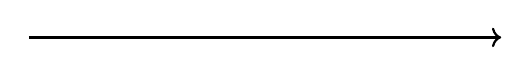
\begin{tikzpicture}\draw[->,thick] (0,0) -- (6,0);\end{tikzpicture}\end{center}\vfill\null\newpage
% tikz-1.5pt
\null\vfill\begin{center}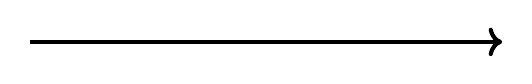
\begin{tikzpicture}\draw[->,line width=1.5pt] (0,0) -- (6,0);\end{tikzpicture}\end{center}\vfill\null\newpage
% tikz-stealth
\null\vfill\begin{center}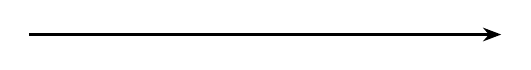
\begin{tikzpicture}\draw[-{Stealth},thick] (0,0) -- (6,0);\end{tikzpicture}\end{center}\vfill\null\newpage
% tikz-latex
\null\vfill\begin{center}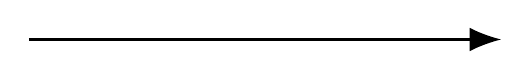
\begin{tikzpicture}\draw[-{Latex[length=4mm]},thick] (0,0) -- (6,0);\end{tikzpicture}\end{center}\vfill\null\newpage
% tikz-3pt
\null\vfill\begin{center}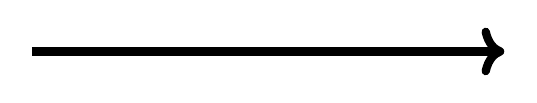
\begin{tikzpicture}\draw[->,line width=3pt] (0,0) -- (6,0);\end{tikzpicture}\end{center}\vfill\null\newpage
\end{document}
